\newpage
\section{Реализация.}
Описанные к главах \ref{chapter:reconstruction_with_rtti} и \ref{chapter:reconstruction_without_rtti} алгоритмы были рассмотрены в применении к версии 9.0.30729.1 компилятора MSVC, и версии 4.2.4 компилятора GCC.

Как было сказано в главе \ref{chapter:problem}, целью данной работы является разработка и реализация методов восстановления объектных структур данных из низкоуровневого представления программ, написанных на языке Си++, для компиляторов GCC и MSVC. Для того, чтобы применить разработанные в главах \ref{chapter:reconstruction_with_rtti} и \ref{chapter:reconstruction_without_rtti} методы к исполняемому файлу, этот файл необходимо дизассемблировать. К настоящему времени проблема дизассемблирования является достаточно хорошо исследованной, и в данной работе не рассматривается. Существует множество различных инструментов для решения этой проблемы, и для поэтому для дизассемблирования исполняемых файлов был использован один из таких инструментов --- интерактивный дизассемблер IDA Pro \cite{idapro}. Описание основных возможностей этого дизассемблера и сравнение его с другими аналогичными по функциональности программными продуктами приведено ниже.


\subsection{Интерактивный дизассемблер IDA Pro}\label{chapter:idapro}
IDA Pro, Interactive Disassembler Pro --- интерактивный дизассемблер, который широко используется для решения задач обратного проектирования. IDA Pro до определенной степени умеет автоматически выполнять анализ, разделяя код и данные, выделяя функции и {\it адаптеры} в потоке инструкций и распознавая стандартные библиотечные функции. Отличительной особенностью IDA Pro является возможность интерактивного взаимодействия с пользователем. В начале исследования дизассемблер выполняет автоматический анализ программы, а затем пользователь с помощью интерактивных средств начинает давать осмысленные имена, комментировать, создавать сложные структуры данных и другим образом добавлять информацию в листинг, генерируемый дизассемблером, пока не станет ясно, что именно делает исследуемая программа.

Дизассемблер имеет консольную и графическую версии, поддерживает большое количество форматов исполняемых файлов, в том числе PE-COFF\footnote{Portable Executable and Common Object File Format, используется в Windows.}, ELF\footnote{Executable and Linkable Format, используется в Linux и большинстве операционных систем семейства BSD.}, Mach-O\footnote{Mach Object, используется в Mac OS X.} и другие \cite{idaproformats}, позволяет анализировать код для более чем пятидесяти семейств процессоров, а также байт-код виртуальных машин Java и .NET \cite{idaproproc}.

IDA Pro имеет модульную архитектуру, что позволяет добавлять в дизассемблер новую функциональность с помощью созданных пользователями плагинов. Примером такого плагина является система Hex-Rays, строящая схему исследуемой программы на Си-подобном языке. Для решения задач меньшего масштаба в IDA Pro встроен похожий на Си язык программирования IDC. Также, воспользовавшись плагинами IDAPython \cite{idapython} или IDARub \cite{idarub}, возможно написание скриптов на python и ruby соответственно. Для скриптов, написанных на языках IDC, python, или ruby, IDA Pro предоставляет большой набор средств для доступа к анализируемому файлу и функциональности дизассемблера. К таким средствам в частности относятся:

\begin{itemize}
\item Простая навигация по анализируемому файлу с использованием виртуальных адресов, а не смещений относительно начала файла.
\item Удобный доступ как к бинарному, так и к разобранному на инструкции представлению программы.
\item Возможность вносить изменения в результаты автоматического анализа.
\item Возможность дизассемблировать произвольную последовательность байт, с проверкой на корректность возможного выполнения полученных инструкций.
\item Доступ к встроенным в IDA Pro средствам анализа. В частности, с использованием стандартных функций IDC можно выделять подпрограммы в потоке инструкций и определять размер {\it стекового фрейма} функции и его составляющих --- параметров, сохраненных регистров, и локальных переменных.
\item Возможность использования поддерживаемой IDA Pro базы перекрестных ссылок для получения адресов всех локаций, каким-либо образом ссылающихся на данную.
\end{itemize}

Использование некоторых из этих средств существенно упрощает решение описанных в главах \ref{chapter:reconstruction_with_rtti} и \ref{chapter:reconstruction_without_rtti} задач анализа ассемблерного представления программы, так как:
\begin{itemize}
\item Для поиска таблиц виртуальных функций необходимо иметь возможность находить адреса всех локаций, каким-либо образом ссылающихся на данную, как это описано в главе \ref{chapter:finding_rtti_structures}.
\item Для применения утверждений \ref{stmt:param_size} и \ref{stmt:param_size_2}, описанных в главе \ref{chapter:param_analysis}, необходимо иметь возможность определять суммарный размер параметров функции по ее эпилогу.
\item Информация о типах времени выполнения имеет сложную структуру, как это описано в главах \ref{chapter:rtti_in_gcc} и \ref{chapter:rtti_in_msvc}, и потому для извлечения этой информации из ассемблерного листинга необходимо иметь возможность навигации по нему с использованием виртуальных адресов.
\end{itemize}

В качестве альтернатив интерактивному дизассемблеру IDA Pro были рассмотрены программные продукты SoftICE и OllyDbg.

SoftICE --- отладчик режима ядра для Microsoft Windows. Программа предназначена для работы на низком уровне операционной системы Windows так, чтобы операционная система не распознавала работу отладчика \cite{boldewin06}. В отличие от отладчиков, работающих в режиме пользователя, SoftICE может остановить все операции в Windows, что очень важно для отладки драйверов. Поддержка SoftICE была приостановлена разработчиками в 2007 году, но не смотря на это, он все еще широко используется. Существует набор средств для создания плагинов для SoftICE. Однако из-за того, что SoftICE работает в режиме ядра, написание плагинов для него становится чрезвычайно сложной задачей, сравнимой с написанием драйверов, работающих в режиме ядра. И если драйвера, работающие в режиме ядра, можно отлаживать с помощью SoftICE, то плагины для SoftICE отлаживать таким способом нельзя. Существующие же плагины для SoftICE, позволяющие использовать скриптовые языки программирования для реализации дополнительной функциональности, имеют весьма ограниченные возможности \cite{softicescripting}.

OllyDbg --- бесплатный 32-битный отладчик для операционных систем семейства Windows, предназначенный для анализа и модификации исполняемых файлов и библиотек, работающих в режиме пользователя. Работа в режиме пользователя в частности означает, что с помощью OllyDbg невозможно отлаживать драйвера, работающие в привилегированном режиме. OllyDbg отличается простым интерфейсом, интуитивной подсветкой специфических структур кода, простотой в установке и запуске. Из особенностей OllyDbg следует выделить \cite{ollydbg}:

\begin{itemize}
\item Поддержку процессоров семейства x86. Расширения SSE2, SSE3, SSE4 не поддерживаются.
\item Анализатор кода, распознающий процедуры, циклы, ветвления, таблицы, константы и текстовые строки.
\item Развернутую система поиска: поиск всех возможных констант, команд, последовательностей команд, текстовых строк и ссылок в коде на данный адрес.
\item Эвристический анализ стека, распознавание адресов возврата в родительскую процедуру.
\item Возможность написания плагинов для расширения имеющейся функциональности. В частности, существует плагин OllyScript, позволяющий писать расширения для OllyDbg на похожем на ассемблер языке программирования.
\end{itemize}

Одним из недостатков системы плагинов OllyDbg является невозможность работы в коде плагинов с подсистемой поиска. Это означает, что поиск всех ссылок в коде на данный адрес необходимо реализовывать самостоятельно. Также несмотря на то, что кроме OllyScript существуют плагины, поддерживающие другие скриптовые языки программирования, такие как python \cite{ollypython}, многие из них недостаточно документированы или уже не поддерживаются авторами.

В результате сравнения возможностей перечисленных программных продуктов было выяснено, что предоставляемые интерактивным дизассемблером IDA Pro средства расширения функциональности являются более простыми в использовании, более документированными, и предоставляющими большие возможности, чем аналогичные средства отладчиков OllyDbg и SoftICE. Написание необходимых алгоритмов с использованием OllyDbg или SoftICE возможно, однако это потребовало бы реализации части той функциональности, которую предоставляет IDA Pro для расширений, реализованных на IDC или python.



\subsection{Программная реализация алгоритмов анализа, использующих информацию о типах времени выполнения}\label{chapter:impl_with_rtti}
Было разработано приложение crec\footnote{от англ. Class hierarchy REConstruction}, в котором были реализованы описанные в главах \ref{chapter:reconstruction_with_rtti} и \ref{chapter:reconstruction_without_rtti} методы восстановления объектных структур данных. Часть этого приложения была реализована на встроенном в интерактивный дизассемблер IDA Pro языке программирования IDC, часть --- на языке Си++.

В случае присутствия информации о типах времени выполнения часть crec, реализованная на языке IDC, анализирует ассемблерный листинг, полученный путем дизассемблирования исполняемого файла дизассемблером IDA Pro, и извлекает из него структуры, содержащие эту информацию. Поиск этих структур производится с использованием алгоритма, описанного в главе \ref{chapter:finding_rtti_structures}. Извлеченные структуры сохраняются в файл в формате XML.

Этот файл является входным для реализованной на языке Си++ части crec. По извлеченной информации о типах времени выполнения эта часть восстанавливает иерархию полиморфных классов программы. Результатом работы этой части является входной файл для утилиты dot из пакета GraphViz \cite{graphviz} с описанием графа, заданного восстановленной иерархией классов. Утилита dot по входному описанию графа строит его графическое представление. Таким образом, с использованием разработанного приложения crec, по ассемблерному листингу исходной Си++-программы, использующей информацию о типах времени выполнения, можно получить графическое представление ее иерархии классов.

%, с использованием которой можно восстановить иерархию классов программы
%Эта часть применяет алгоритмы, описанные в главах \ref{chapter:reconstruction_with_rtti} и \ref{chapter:reconstruction_without_rtti}, и таким образом восстанавливает иерархию классов.

%Пример работы приложения crec приведен ниже.

\begin{figure}[htb!]
\centering
\includegraphics[width=0.8\textwidth]{images/doxy_objtree_our.png}
\caption{Графическое представление фрагмента иерархии полиморфных классов программы doxygen, полученное с использованием приложения crec путем анализа информации о типах времени выполнения.}
\label{fig:doxy_objtree_our}
\end{figure}

\begin{figure}[htb!]
\centering
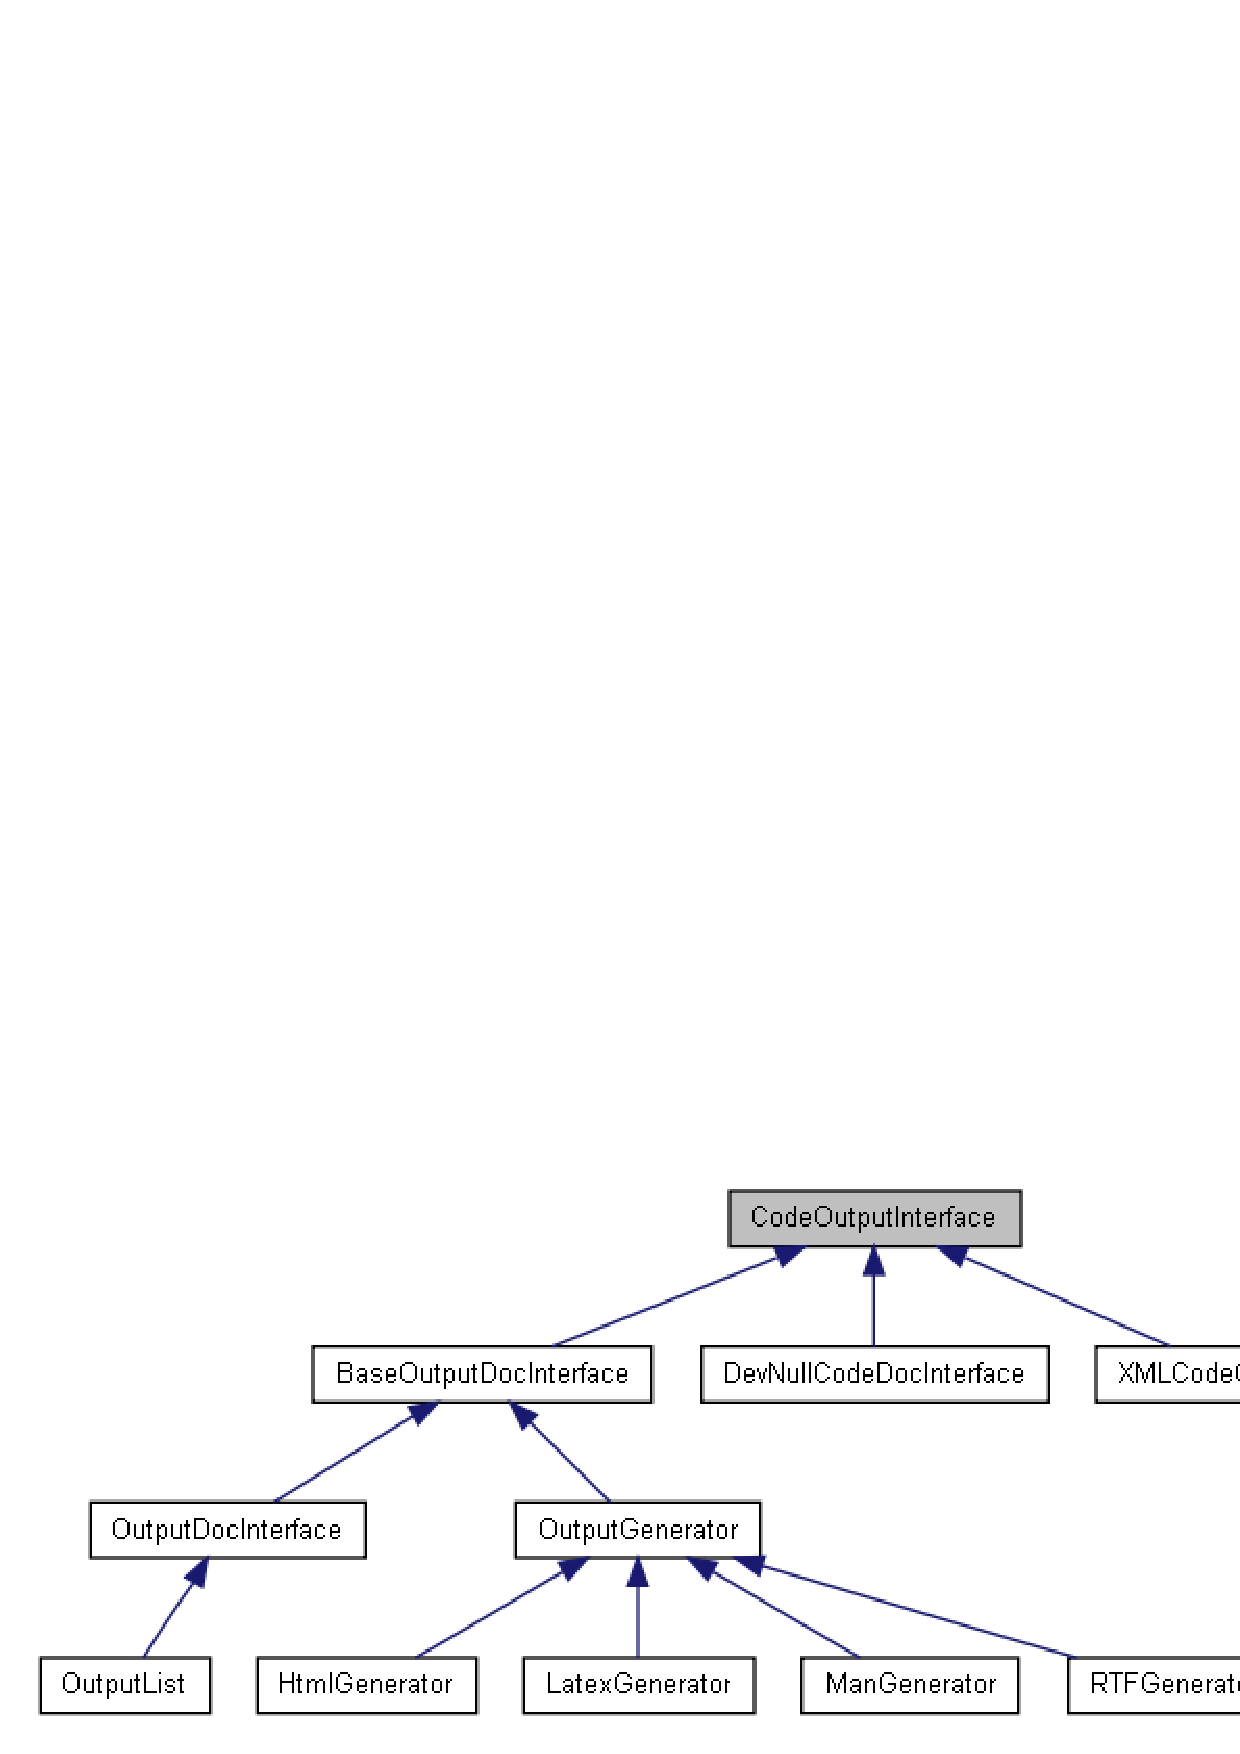
\includegraphics[width=0.8\textwidth]{images/doxy_objtree_doxy.png}
\caption{Графическое представление фрагмента иерархии полиморфных классов doxygen, полученное путем анализа исходного кода с помощью программы doxygen.}
\label{fig:doxy_objtree_doxy}
\end{figure}

Пример графического представления иерархии полиморфных классов, восстановленной с использованием приложения crec, приведен на рис. \ref{fig:doxy_objtree_our}. В качестве анализируемой программы использовалась система документирования исходных кодов doxygen. Одной из причин использования doxygen в качестве анализируемой программы является то, что doxygen распространяется с открытыми исходными кодами, что упрощает проверку корректности результатов восстановления. Также изучение исходных кодов doxygen показало, что в некоторых методах используется оператор \lstinline{dynamic_cast<>}, и поэтому для правильной работы этой программы она должна была быть скомпилирована с поддержкой информации о типах времени выполнения. Целью анализа являлось восстановление иерархии полиморфных классов. Для этого необходима информация о:
\begin{itemize}
\item Компиляторе, с использованием которого был получен исполняемый файл;
\item Формате RTTI структур, который используется этим компилятором.
%\item Извлечь RTTI структуры из исполнимого файла с использованием описанного выше алгоритма.
%\item Построить иерархию использованных в приложении полиморфных классов путем анализа извлеченных RTTI структур.
\end{itemize}

В результате применения методов, описанных в главе \ref{chapter:rtti_extraction}, было выяснено, что doxygen 1.5.8 для Windows скомпилирован компилятором MSVC, формат RTTI структур для которого был описан в главе \ref{chapter:rtti_in_msvc}. С использованием написанной на языке IDC части crec был проанализирован ассемблерный листинг. С использованием написанной на Си++ части crec была восстановлена полная иерархия полиморфных классов программы doxygen, состоящая из 444 классов. На рис. \ref{fig:doxy_objtree_our} приведено графическое представление фрагмента восстановленной иерархии полиморфных классов, а на рис. \ref{fig:doxy_objtree_doxy} --- графическое представление того же фрагмента, полученное путем анализа исходного кода. Как видно, фрагменты иерархии совпадают.

В результате сравнения иерархии полиморфных классов doxygen, построенной путем анализа исходного кода, с иерархией, восстановленной с использованием приложения crec, было выяснено, что эти иерархии совпадают.



\subsection{Программная реализация алгоритмов анализа, не использующих информацию о типах времени выполнения}
В приложении crec также были реализованы методы восстановления иерархий полиморфных классов для случая отсутствия информации о типах времени выполнения, описанные в главе \ref{chapter:reconstruction_without_rtti}. Извлечение информации, необходимой для построения ограничений с использованием утверждений \ref{stmt:first_good}-\ref{stmt:last_good}, производится в части crec, реализованной на языке IDC. Анализ извлеченной информации с использованием описанных в главе \ref{chapter:reconstruction_without_rtti} методов производится в части crec, реализованной на языке Си++. Результатом работы приложения crec является входной файл для утилиты dot из пакета GraphViz, как это описано в главе \ref{chapter:impl_with_rtti}.

\begin{figure}[htb!]
\centering
\includegraphics[width=0.8\textwidth]{images/doxy_objtree_nortti.png}
\caption{Графическое представление фрагмента иерархии полиморфных классов программы doxygen, полученное с использованием приложения crec без использования информации о типах времени выполнения.}
\label{fig:doxy_objtree_nortti}
\end{figure}

\begin{figure}[htb!]
\centering
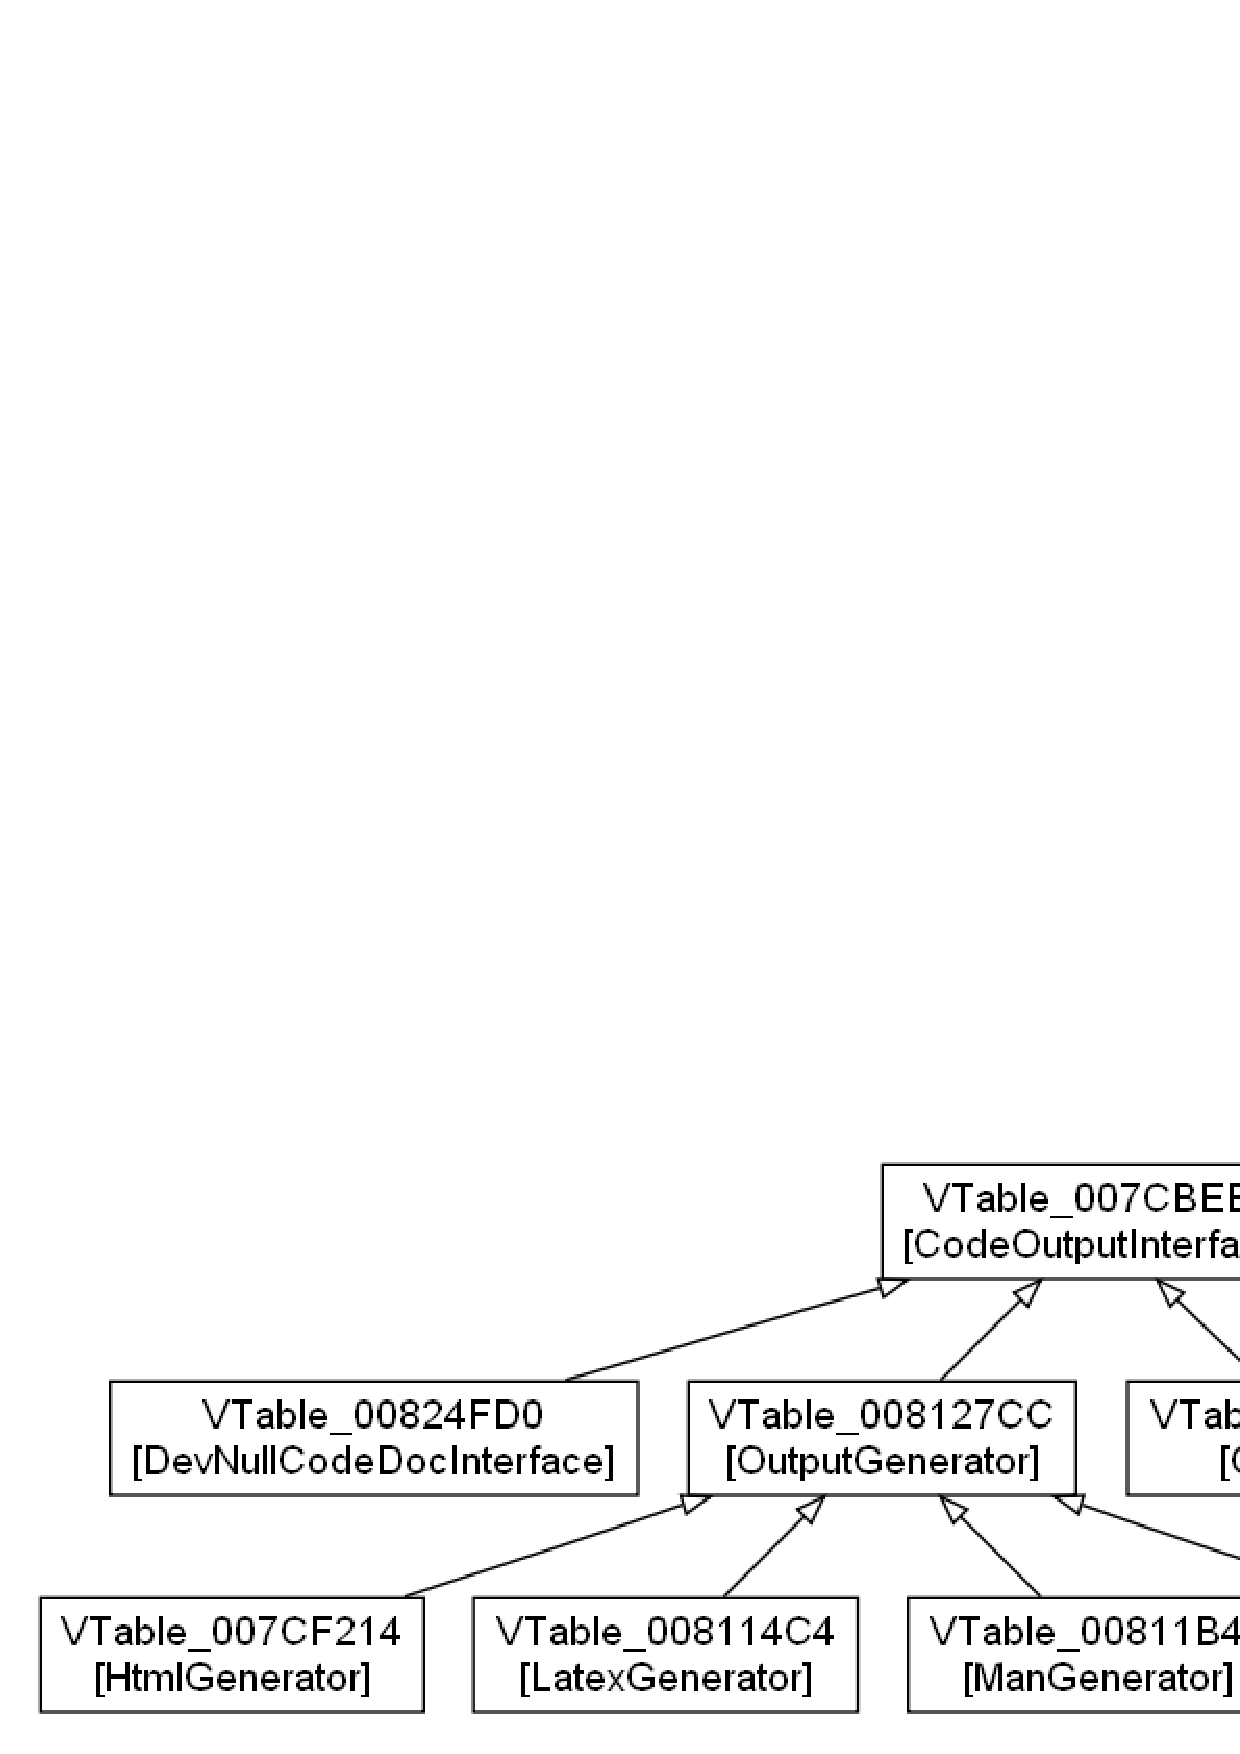
\includegraphics[width=0.8\textwidth]{images/doxy_objtree_nortti_label.png}
\caption{Графическое представление иерархии классов, представленной на рис. \ref{fig:doxy_objtree_nortti}, с сопоставленными классам реальными именами.}
\label{fig:doxy_objtree_nortti_label}
\end{figure}

Пример графического представления иерархии полиморфных классов, восстановленной с использованием приложения crec, представлен на рис. \ref{fig:doxy_objtree_nortti}. Также, как и в главе \ref{chapter:impl_with_rtti}, в качестве анализируемой программы использовалась система документирования исходных кодов doxygen. Анализируемый исполнимый файл был получен путем компиляции doxygen без поддержки информации о типах времени выполнения компилятором MSVC. При компиляции без информации о типах времени выполнения имена классов не попадает в исполнимый файл, и поэтому все классы на рис. \ref{fig:doxy_objtree_nortti} имеют автоматически сгенерированные имена.

Для проверки корректности восстановления система doxygen была скомпилирована еще раз с поддержкой информации о типах времени выполнения. Для исполнимого файла, полученного путем компиляции с использованием информации о типах времени выполнения, иерархия полиморфных классов была восстановлена так, как это описано в главе \ref{chapter:impl_with_rtti}. Путем сравнения виртуальных функций каждой таблице виртуальных функций из ассемблерного листинга исполнимого файла, полученного компиляцией без поддержки информации о типах времени выполнения, была поставлена в соответствие таблица виртуальных функций из ассемблерного листинга исполнимого файла, полученного компиляцией с поддержкой информации о типах времени выполнения. Таким образом, для каждой таблицы виртуальных функций из ассемблерного листинга исполнимого файла, полученного компиляцией без поддержки информации о типах времени выполнения, было получено имя соответствующего ей класса. На рис. \ref{fig:doxy_objtree_nortti_label} представлен фрагмент иерархии, соответствующий представленному на рис. \ref{fig:doxy_objtree_nortti} фрагменту иерархии, но с сопоставленными классам реальными именами.

Представленный на рис. \ref{fig:doxy_objtree_nortti_label} восстановленный фрагмент иерархии соответствует фрагменту, изображенному на рис. \ref{fig:doxy_objtree_doxy}. Как видно, фрагменты иерархии отличаются. Это объясняется тем, что классы \lstinline{BaseOutputDocInterface} и \lstinline{OutputDocInterface}, присутствующие в фрагменте иерархии, изображенном на рис. \ref{fig:doxy_objtree_doxy}, не перекрывают унаследованные ими виртуальные функции, а лишь добавляют новые чисто виртуальные функции, и потому компилятором для этих классов не была сгенерирована таблица виртуальных функций.

В результате сравнения иерархии полиморфных классов doxygen, восстановленной с помощью приложения crec без использования информации о типах времени выполнения, с иерархией, построенной путем анализа исходного кода, было выяснено, что восстановление иерархии было произведено корректно.














